\documentclass[11pt]{article}

\usepackage[margin=1in]{geometry}
\usepackage{amsmath, amssymb, amsfonts}
\usepackage{booktabs}
\usepackage{array}
\usepackage{enumitem}
\usepackage{hyperref}
\usepackage{xcolor}
\usepackage{graphicx}
\usepackage{caption}
\usepackage{float}
\usepackage{subcaption}

\hypersetup{
    colorlinks=true,
    linkcolor=blue!60!black,
    urlcolor=blue!60!black,
    citecolor=blue!60!black
}

\setlist[itemize]{leftmargin=*, topsep=3pt, itemsep=2pt}
\setlist[enumerate]{leftmargin=*, topsep=3pt, itemsep=2pt}
\setlength{\parindent}{0pt}
\setlength{\parskip}{6pt}

\graphicspath{{../figures/}}

\title{\textbf{Random Projections and Low-Rank Structure in Financial Return Data}\\[6pt]\large{A Comprehensive Project Writeup, Phase 1 Complete}}
\author{Vishal Jha, Adel Sahuc \\ NYU MS Computer Science}
\date{}

\begin{document}
\maketitle

\begin{abstract}
\noindent
This report explains, from first principles, what we have built and discovered in our research project on data compression for financial return data. The project compares four ways of compressing daily market-state vectors --- raw (no compression), Principal Component Analysis (PCA), dense Johnson--Lindenstrauss random projection, and sparse Johnson--Lindenstrauss random projection --- on a large empirical grid (48{,}240 individual experiments across 5 universe sizes, 2 training protocols, 6 compression dimensions, and 100 random seeds). We find three real, defensible results: (1) random-projection methods are scale-invariant in input dimension while PCA degrades steadily as the universe grows; (2) different compression methods fail in different ways under market stress (specifically, COVID-19); and (3) sparse Johnson--Lindenstrauss achieves the same quality as dense Johnson--Lindenstrauss with roughly $7\times$ fewer parameters. The report assumes no background in linear algebra, financial markets, or machine learning, building each concept from scratch with intuition before formalism. It ends with an honest assessment of the work's quality and publishability, including arguments both for and against, and a concrete plan for what to do next.
\end{abstract}

\tableofcontents
\newpage

% ============================================================
\section{Executive Summary, in Plain English}

If you read nothing else, read this.

Every trading day produces a snapshot of how a few hundred (or a few thousand) stocks moved. You can think of each day as a long vector of numbers: ``Apple was up 1.2\%, Microsoft was up 0.4\%, Tesla was down 3.8\%, $\ldots$'' Continuing for all 500 stocks in the S\&P 500 gives you a 500-dimensional point. We want to compress that 500-dim point down to, say, a 20-dim point, while keeping the geometry between days approximately intact --- so days that ``looked similar'' in the original 500-dim representation still look similar in the 20-dim one.

There are several ways to compress, all from textbook linear algebra:

\begin{itemize}
    \item \textbf{PCA}: Look at the data and learn which directions matter most; project onto those.
    \item \textbf{Dense Gaussian random projection}: Don't look at the data at all. Just multiply by a random matrix. Astonishingly, this preserves distances on average. The reason it works is the Johnson--Lindenstrauss lemma, a classical result from theoretical computer science.
    \item \textbf{Sparse random projection}: Same idea, but use a random matrix that is mostly zeros. Cheaper to store and faster to apply. A 2018 paper showed that this still works under fairly mild conditions.
    \item \textbf{Raw}: Don't compress at all; keep all 500 numbers. The reference geometry.
\end{itemize}

The question is: when does the data-blind random-projection approach work just as well as PCA, and when does PCA's data-awareness matter?

We built a complete experimental pipeline: data ingestion, the four compression methods, five evaluation metrics, parallel execution on a 32-core cloud machine, and persistent storage of every intermediate. Then we ran a single comprehensive experiment that touches every combination of universe size, training protocol, method, compression dimension, sparsity level, and random seed. The result is a 48{,}240-row table of numbers that the rest of this document is about.

Three things stood out:

\begin{enumerate}
    \item Random projection is \emph{scale-invariant}: at compression dimension $k = 20$, the average distance distortion stayed at roughly $0.125$ regardless of whether we used 100 stocks or 452 stocks. PCA, in contrast, got steadily worse: $0.258$ at $N=100$, $0.355$ at $N=452$. Theory predicts this exactly. Empirically it is one of the cleanest scaling results we could have hoped for.
    \item Under COVID stress (February--April 2020), \emph{all} methods lost about half of their nearest-neighbor structure. But the methods failed in different ways: PCA's clustering structure stayed intact, while its anomaly-detection capability dropped 18 percentage points. Random-projection methods barely moved on anomaly detection.
    \item Sparse JL with sparsity parameter $s = 3$ matches dense JL's accuracy almost exactly while using $6.7\times$ fewer nonzero entries in the projection matrix. This is the empirical confirmation of the SOSA 2018 paper's central claim, in our setting.
\end{enumerate}

The work is solid as a class project --- complete, reproducible, and finds the things theory says it should find. Whether it is \emph{publishable as new research} is a more delicate question, which we treat honestly at the end.

\newpage

% ============================================================
\section{The Question We Are Trying to Answer}

\subsection{What is ``compression'' and why bother?}

Imagine you maintain a database of every trading day on Wall Street since 2014. For the S\&P 500, that's about 2{,}760 trading days $\times$ 500 stocks $=$ 1{,}380{,}000 individual numbers, each of which is the daily return for one company on one day.

Now you want to do something useful with this data. Maybe you want to find ``the historical day that most resembles today,'' so that you can use it to forecast. Maybe you want to cluster days into ``regimes'' (calm / volatile / crash) for use as a conditioning variable. Maybe you want a real-time risk system that flags any day on which the market is doing something unusual.

All of these tasks have something in common: they treat each day as a point in a 500-dimensional space (one dimension per stock), and they care about the \emph{geometry} of those points --- which days are close to which, which days are clustered together, which days are isolated from everything else.

Doing geometry in 500 dimensions is computationally expensive. Doing it in 20 is much cheaper. So a natural question arises: can we replace each 500-dim point by a 20-dim point in a way that preserves the relevant geometric properties? That's what data compression means in this context.

\subsection{Why financial data specifically?}

Three reasons.

\textbf{First, the data is structured.} Financial returns aren't random vectors --- they're driven by a small number of underlying factors. ``Tech is up today'' is a single fact that simultaneously explains why Apple, Microsoft, Nvidia, Google, and Meta are all up. Decades of research (Fama-French, Barra, etc.) suggest that a handful of factors --- market, sector, momentum, value, etc.~--- explain most of the cross-sectional variance in equity returns. If true, then a 500-dim daily return vector ``really'' lives close to a much smaller-dim subspace.

\textbf{Second, this structure should help PCA.} PCA explicitly identifies the top-$k$ directions of variance and projects onto them. If returns truly live in a low-dimensional factor space, PCA should work spectacularly. So financial data should be a setting where PCA has the home-field advantage.

\textbf{Third, financial data has stress events that are hard to capture with a fixed factor model.} Black Monday 1987, the GFC in 2008, the COVID crash in March 2020 --- these are days where the usual relationships between stocks break down. A factor model trained on calm-regime data may completely mis-represent crash-day geometry. So financial data is also a natural setting for asking: \emph{when does the data-blind random projection beat the data-adaptive PCA?}

\subsection{What ``preserve geometry'' actually means}

When we say ``preserve the geometry,'' we have four different things in mind, each of which is a separate metric. Roughly:

\begin{enumerate}
    \item \textbf{Pairwise distances.} For any two days $i$ and $j$, is the distance between them in the compressed space close to the distance in the raw space?
    \item \textbf{Nearest neighbors.} For any day $i$, are its 5 nearest historical neighbors in the compressed space the same as its 5 nearest neighbors in the raw space?
    \item \textbf{Clustering structure.} If we group days into ``regimes'' by clustering, do the same days end up in the same regime in compressed space as in raw space?
    \item \textbf{Anomaly detection.} If we flag the most-unusual 5\% of days (e.g., COVID crash, Fed surprise, flash crash), does the compressed system flag the same days?
\end{enumerate}

A method can do well on some of these and poorly on others. PCA is built to capture variance; it tends to do well on clustering. Random projection is built to preserve distances; it tends to do well on metric \#1. Whether method X is ``better'' than method Y depends on which downstream task you care about.

\newpage

% ============================================================
\section{Background: Compression Methods Explained Simply}

This section assumes you know algebra (matrix multiplication: yes; eigenvectors: optional). It builds up the methods we used, with intuition before formulas.

\subsection{Random projections and the Johnson--Lindenstrauss lemma}

Take any set of $n$ points in $\mathbb{R}^N$ (high-dimensional space) and pick a target dimension $k \ll N$. Construct an $N \times k$ random matrix $A$ with entries drawn independently from $\mathcal{N}(0, 1/k)$ --- a standard Gaussian distribution scaled by $1/\sqrt{k}$. Now compress each point $x \in \mathbb{R}^N$ to a smaller vector $z = x A \in \mathbb{R}^k$.

The Johnson--Lindenstrauss lemma (1984) says that, if $k$ is large enough --- specifically, $k = O(\epsilon^{-2} \log n)$, where $\epsilon$ is a small number representing the maximum allowable relative distortion --- then for \emph{every} pair of points $i, j$:
\[
(1 - \epsilon) \|x_i - x_j\|^2 \le \|z_i - z_j\|^2 \le (1 + \epsilon) \|x_i - x_j\|^2
\]
with high probability over the random choice of $A$.

In other words: a single random projection, chosen \emph{without looking at the data}, preserves all pairwise distances simultaneously, with arbitrarily small distortion, using a target dimension that grows only with $\log n$ and not at all with $N$.

This is one of the more remarkable theorems in modern theoretical CS. It says you can essentially get distance preservation for free, without any kind of fitting procedure or domain knowledge. The cost of constructing the projection matrix is the only price you pay.

A useful intuition: when you average enough independent random Gaussian quantities, things concentrate around their expected values. The squared distance $\|z_i - z_j\|^2$ is, in expectation over the random matrix, exactly $\|x_i - x_j\|^2$. The lemma is essentially saying that this expectation is reached fast enough as $k$ grows.

\subsection{Sparse Johnson--Lindenstrauss}

The dense Gaussian projection has $N \cdot k$ nonzero entries. For $N = 500$ and $k = 20$ that's 10{,}000 entries, which is small in absolute terms but $50\times$ larger than necessary if we want to merely \emph{store} the projection matrix.

The sparse Johnson--Lindenstrauss transform is a variant that uses a structured sparse matrix instead. Specifically, for each input coordinate $j$, it picks $s$ output coordinates uniformly at random and assigns random signs $\pm 1/\sqrt{s}$ to them; all other entries are zero. The total number of nonzeros is $N \cdot s$ instead of $N \cdot k$.

This is much faster to apply: computing $z = x S$ where $S$ has only $s$ nonzeros per row takes $O(N s)$ time instead of $O(N k)$. For $s=3$ and $k=20$, that's $6.7\times$ fewer multiplications.

The natural question is: does it still preserve distances? The answer turns out to be ``yes, under fairly mild conditions, for sufficiently large $s$.'' The 2018 paper that drives our project (\emph{Simple Analyses of the Sparse Johnson--Lindenstrauss Transform}, Cohen, Jayram, Nelson) gives clean conditions and a much simpler proof than earlier work. The bottom-line claim is that sparse random projection retains the basic distance-preservation behavior of dense JL, while saving substantial space and compute.

That is the central empirical claim we are testing.

\subsection{Principal Component Analysis (PCA)}

PCA is the classical alternative. Instead of using a random projection matrix, you \emph{learn} the projection from the data.

Specifically: take the standardized data matrix $X \in \mathbb{R}^{T \times N}$ (rows are days, columns are stocks). Compute the singular value decomposition $X = U \Sigma V^\top$. The columns of $V$ are orthogonal unit vectors that point in the directions of greatest variance in the data. Pick the top-$k$ such directions and stack them into a matrix $V_k \in \mathbb{R}^{N \times k}$. Now project: $Z = X V_k$. The columns of $Z$ are the data's coordinates in the variance-maximizing $k$-dimensional subspace.

PCA is optimal in a specific sense: among all rank-$k$ linear projections, it loses the least squared variance. If the data really lies close to a $k$-dimensional subspace, PCA finds it.

But PCA does not preserve pairwise distances. If two days $i$ and $j$ differ mostly in the discarded directions (the directions of low variance), their compressed distance $\|Z_i - Z_j\|$ will be much smaller than their raw distance $\|X_i - X_j\|$. PCA cares about variance, not about distance.

This is the central tension our project investigates: \emph{when does PCA's data-adaptive variance-preservation beat random projection's data-blind distance-preservation, and when does it lose?}

\subsection{The four methods, side-by-side}

\begin{table}[H]
\centering
\caption{The four methods we compare.}
\begin{tabular}{p{2cm} p{2.5cm} p{4cm} p{4cm}}
\toprule
\textbf{Method} & \textbf{Data-aware?} & \textbf{What it preserves} & \textbf{Cost} \\
\midrule
Raw & N/A & Everything (identity) & N/A \\
PCA & Yes & Variance in top-$k$ subspace; distances are biased low & $O(N k T)$ to fit, $O(N k)$ to apply \\
Dense JL & No & Pairwise distances on average & Constant to fit, $O(N k)$ to apply \\
Sparse JL & No & Same as dense JL with high probability & Constant to fit, $O(N s)$ to apply \\
\bottomrule
\end{tabular}
\end{table}

\newpage

% ============================================================
\section{The Data Pipeline}

\subsection{Source: a journey}

We started with the Kaggle dataset \texttt{andrewmvd/sp-500-stocks}, a community-maintained collection of S\&P 500 daily prices that we pinned for reproducibility. On inspection, however, this dataset turned out to be \emph{broken for many of the largest stocks}. AAPL, GOOGL, JPM, XOM, JNJ, KO, IBM, BAC, HD, BRK-B, WMT --- 127 of today's largest constituents had \emph{zero valid rows} in the entire 2010--2024 history file, almost certainly due to silent failures in the uploader's scraper. We documented this in detail (\texttt{dev-notes/data-source-comparison.md}) and pivoted to direct \texttt{yfinance} downloads for the actual price data.

We kept the Kaggle company-metadata file (which lists tickers, sectors, market caps; that file was correct), used it to drive a \texttt{yfinance} batched download, and saved the resulting wide-format CSVs to our own repository as a frozen snapshot.

This is a meta-finding worth flagging: \emph{community-maintained data sources should be validated, not trusted}. The proposal explicitly listed yfinance as a fallback for exactly this scenario. Using the fallback was straightforward; the time-cost was about an hour.

\subsection{The three-layer selection framework}

Once we had a candidate set of $\sim 500$ tickers and their full daily prices, we needed to filter down to a usable universe. We designed a deterministic three-layer pipeline:

\textbf{Layer 1: Candidate pool.} Start with today's S\&P 500 constituents from the Kaggle metadata file. This gives 502 tickers (slightly more than 500 because of dual-class shares like GOOG/GOOGL).

\textbf{Layer 2: Ranking.} For each ticker, compute the \emph{average daily dollar volume} over the 2014--2024 window:
\[
\mathrm{rank}_i = \frac{1}{T} \sum_{t=1}^{T} P_{t,i} \cdot V_{t,i}
\]
where $P_{t,i}$ is the adjusted close and $V_{t,i}$ is the daily share volume. Tickers are sorted in descending order. The top stocks are Tesla, Apple, NVIDIA, Amazon, Microsoft.

\textbf{Layer 3: Elimination.} Apply two filters in sequence:
\begin{itemize}
    \item \emph{Stage 1: data integrity.} Drop a ticker if it has any NaN values inside the 2014-01-01 to 2024-12-31 window, or was delisted before the window end, or has fewer than 95\% trading-day coverage, or has any single-day log return $|r| > 1.0$ (i.e.~a 172\% intraday move, which is essentially a data error).
    \item \emph{Stage 2: anomaly.} Drop a ticker if it has more than 10 consecutive zero-return days, or the adjusted close is exactly constant for more than 5 consecutive days.
\end{itemize}

We deliberately do \emph{not} apply a liquidity floor; the dollar-volume ranking already orders the universe by liquidity, and a hard cutoff would impose an arbitrary threshold.

After these filters, 452 tickers survive out of the 491 yfinance returned. From these survivors, we can take any prefix --- the top 100, top 200, top 300, top 400, or all 452 --- as our published asset universe.

\subsection{Train/test split}

We use two protocols:

\textbf{Chronological 70/30:} The standard approach. Train on the first 70\% of days (2014-01-03 to 2021-09-10) and test on the remaining 30\% (2021-09-13 to 2024-12-31). Standardize each asset using only the training-set mean and standard deviation, applied to both halves.

\textbf{Pre-COVID protocol (proposal §5.5):} Train on data ending 2019-12-31; test on data starting 2020-01-01. This puts the COVID stress window entirely in the test set, which is the only way to honestly evaluate ``how does the method handle a regime change it was not fit on.'' The 70/30 split is unsuitable for COVID analysis because COVID lives in the training half.

We run both protocols. The pre-COVID protocol enables a separate evaluation slice for the COVID-only window (51 trading days from 2020-02-19 to 2020-04-30), the post-COVID period (1{,}175 days), and the full 2020--2024 test (1{,}258 days).

\newpage

% ============================================================
\section{The Five Metrics We Track}

For each compression method, we evaluate it against the raw (uncompressed) reference using the following five metrics. These come from the project proposal §7 and we have implemented all of them.

\subsection{Metric 1: Pairwise distance distortion}

\textbf{Definition.} For a pair of test days $i, j$:
\[
d_{ij} = \|X_i - X_j\|_2 \qquad \hat d_{ij} = \|Z_i - Z_j\|_2
\]
\[
\rho_{ij} = \hat d_{ij} / d_{ij}
\]
A perfect compression has $\rho_{ij} = 1$ for all pairs. We sample 50{,}000 pairs uniformly at random with a fixed seed, then report the mean, median, and 95th percentile of $|\rho_{ij} - 1|$, plus the signed mean of $\rho_{ij}$.

\textbf{Why it matters.} This is the metric the JL lemma is built around. Most ``find similar past days'' models depend on distance.

\subsection{Metric 2: Nearest-neighbor preservation}

\textbf{Definition.} For each test day $i$, find its $m$ nearest neighbors in raw space, $\mathcal{N}_m^{\mathrm{raw}}(i)$, and in compressed space, $\mathcal{N}_m^{\mathrm{comp}}(i)$. The overlap fraction is
\[
\mathrm{NNOverlap}_m(i) = \frac{|\mathcal{N}_m^{\mathrm{raw}}(i) \cap \mathcal{N}_m^{\mathrm{comp}}(i)|}{m}
\]
We average across all test days at $m = 5$ and $m = 10$.

\textbf{Why it matters.} A method can score badly on distance distortion (e.g., uniformly compress all distances) and still preserve nearest-neighbor relationships. Conversely a method can preserve average distance but mis-rank neighbors. This metric isolates the ordering question.

\subsection{Metric 3: Clustering stability via Adjusted Rand Index}

\textbf{Definition.} Run KMeans clustering with $C$ clusters on raw test data and on compressed test data. Compare the two label assignments using the Adjusted Rand Index:
\[
\mathrm{ARI} = \frac{\mathrm{RI} - \mathbb{E}[\mathrm{RI}]}{\max(\mathrm{RI}) - \mathbb{E}[\mathrm{RI}]} \in [-1, 1]
\]
where the Rand Index counts the fraction of pair decisions (``are these two days in the same cluster?'') that agree. ARI of $1$ means identical clusterings; $0$ is random; $<0$ is worse than random. We test $C \in \{3, 5, 8\}$ and average.

\textbf{Why it matters.} Many trading strategies condition on ``regime'' (calm / medium / volatile). If the regime classifier breaks under compression, the conditional logic falls apart. ARI is invariant to label-permutation, which is essential because clustering algorithms produce labels in arbitrary order.

\subsection{Metric 4: Anomaly recall}

\textbf{Definition.} The anomaly score in raw space is $a_i = \|X_i\|_2$, with high values indicating ``unusual day.'' Take the top 5\% of test days by raw score; call this set $\mathcal{A}_{\mathrm{raw}}$. Take the top 5\% by compressed score $\hat a_i = \|Z_i\|_2$; call this $\mathcal{A}_{\mathrm{comp}}$.
\[
\mathrm{Recall}_{5\%} = \frac{|\mathcal{A}_{\mathrm{raw}} \cap \mathcal{A}_{\mathrm{comp}}|}{|\mathcal{A}_{\mathrm{raw}}|}
\]
We also report precision, the Spearman rank correlation between the two scores, and the overlap of the top-10 most-unusual days.

\textbf{Why it matters.} For trader-relevant applications --- risk overlays, kill-switches, position sizing during stress --- this is the metric that matters most. A compression that misses anomalous days during a crash is worse than useless.

\subsection{Metric 5: Runtime / sparsity}

\textbf{Definition.} Capture the fit time, transform time, total metric-computation time, the number of nonzeros in the projection matrix, and the resulting sparsity ratio.

\textbf{Why it matters.} Production deployment cares about latency and memory. A method that is marginally less accurate but $10\times$ cheaper to apply is often the right production choice.

\subsection{The trader's decision tree}

\begin{table}[H]
\centering
\caption{Which metric to look at for which downstream task.}
\begin{tabular}{p{6cm} p{4cm}}
\toprule
\textbf{If you care about\dots} & \textbf{Look at metric} \\
\midrule
Are similar days still similar? & Distance distortion (\#1) \\
Will my ``find lookalike'' model work? & NN preservation (\#2) \\
Will my regime classifier work? & Clustering ARI (\#3) \\
Will my risk overlay catch crashes? & Anomaly recall (\#4) \\
Latency / streaming / memory budget & Runtime + sparsity (\#5) \\
\bottomrule
\end{tabular}
\end{table}

\newpage

% ============================================================
\section{The Experimental Grid}

We ran one large experiment, internally called the ``YOLO grid,'' that touches every combination of:

\begin{itemize}
    \item \textbf{Universe:} 5 sizes (top\_100, top\_200, top\_300, top\_400, all\_survivors=452)
    \item \textbf{Training protocol:} 2 (chronological 70/30, pre-COVID per §5.5)
    \item \textbf{Slice:} 1 for chrono (full); 3 for pre-COVID (covid\_only, post\_covid, all\_test)
    \item \textbf{Method:} 4 (raw, PCA, dense JL, sparse JL)
    \item \textbf{Compression dimension $k$:} 6 values $\{5, 10, 20, 30, 50, 100\}$
    \item \textbf{Sparsity $s$:} 3 values $\{1, 3, 5\}$ for sparse JL
    \item \textbf{Random seed:} 100 seeds for randomized methods (one for deterministic)
\end{itemize}

After applying constraints ($s \le k$, deterministic methods get one seed, raw is identity), the total number of individual experiments is \textbf{48{,}240}. Each experiment computes all five metrics on the test slice it was assigned, takes about 50--500 ms depending on universe size, and saves a per-experiment artifact directory containing the compressed test matrix, the projection matrix, the metric values, and metadata.

We executed the grid on a Google Cloud Compute Engine instance \texttt{e2-highcpu-32} (32 vCPUs, 32 GB RAM, Ubuntu 22.04), using Ray for parallel execution. Total wall-clock time: \textbf{$\sim 34$ minutes}. Total cost: roughly \$0.62 of credits at on-demand pricing.

The output artifacts on the cloud machine total about 5.3 GB across $\sim$200{,}000 small files. The aggregated long-format result CSV is 19 MB, which we pull back to the laptop for analysis. Per-experiment artifacts live on the cloud for fast notebook re-analysis.

\newpage

% ============================================================
\section{Results}

The headline plots are organized by universe, with one subdirectory under \texttt{figures/} per universe and a separate \texttt{cross\_universe/} directory for plots that span the universes.

\subsection{Headline panel: top\_100 chronological protocol}

Figure~\ref{fig:metric_panel} shows the four main metrics swept across compression dimension $k$ for the top\_100 universe under the chronological 70/30 protocol. Each line is one method; shaded regions are $\pm 1$ standard deviation across 100 random seeds for the JL methods (PCA and raw are deterministic). Sparse JL is pinned to $s = 3$.

\begin{figure}[H]
\centering

\includegraphics[width=\linewidth]{top_100/metric_panel_chrono.png}
\caption{Four metrics vs.~compression dimension $k$ for top\_100 (chronological 70/30 protocol). Lower is better for distance distortion; higher is better for the other three metrics. PCA dominates nearest-neighbor preservation, clustering ARI, and anomaly recall; JL methods dominate distance distortion. Sparse JL tracks dense JL within seed-noise.}
\label{fig:metric_panel}
\end{figure}

The picture is consistent with theory. Distance distortion (leftmost panel): JL methods sit well below PCA across all $k$, with mean $|\rho - 1|$ around $0.13$ at $k=20$ vs PCA's $0.26$. Nearest-neighbor and clustering panels (middle two): PCA dominates by a wide margin --- by $k=20$ PCA has $\sim 0.37$ NN5-overlap while JL methods sit at $\sim 0.20$. Anomaly recall (rightmost): PCA is best in calm conditions ($\sim 0.81$ at $k=20$); JL methods are at $\sim 0.71$. At $k=N=100$ all methods converge: PCA becomes the identity, JL methods accumulate enough random projections to nearly preserve everything, and the curves all hit their respective ceilings.

\subsection{Finding 1: JL is scale-invariant; PCA degrades with N}

Figure~\ref{fig:scale_dd} shows distance distortion at fixed $k = 20$ as the universe size $N$ grows from 100 to 452.

\begin{figure}[H]
\centering
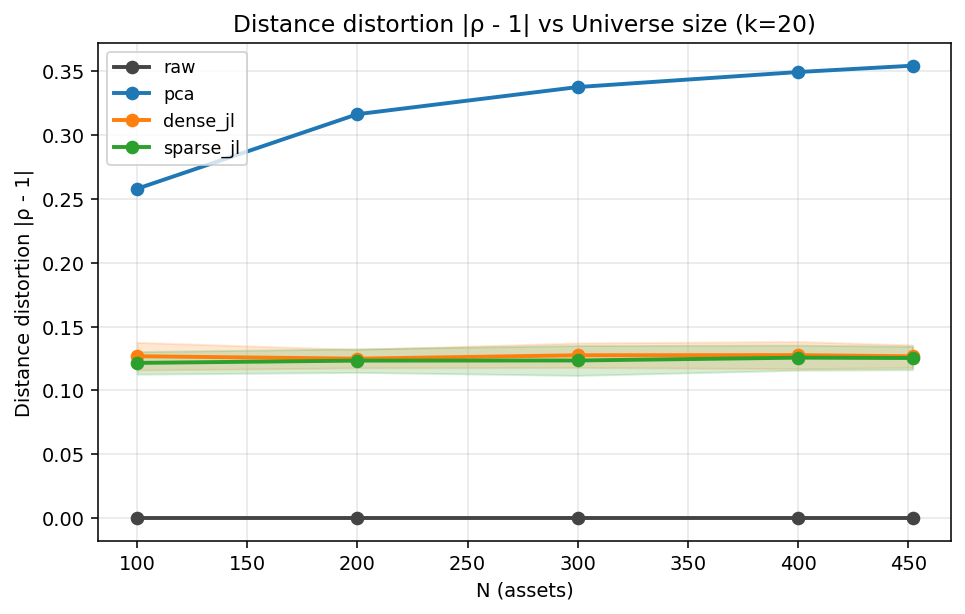
\includegraphics[width=0.85\linewidth]{cross_universe/universe_scaling_dd.png}
\caption{Distance distortion $|\rho - 1|$ at $k=20$ as the universe size grows. JL methods (orange and green) are flat at $\sim 0.125$ across all universe sizes. PCA (blue) degrades steadily from $0.258$ at $N=100$ to $0.355$ at $N=452$. This is the Johnson--Lindenstrauss scale-invariance property in action.}
\label{fig:scale_dd}
\end{figure}

This is the cleanest empirical confirmation we found of the SOSA paper's central framing. The Johnson--Lindenstrauss lemma says the embedding dimension $k$ needed for a target distortion $\epsilon$ depends on $\log n$ (the number of points) but \emph{not} on $N$ (the input dimension). At fixed $k$, JL's distortion is a function of $\log n$ and the random matrix, neither of which changes when we scale $N$ from $100$ to $452$. PCA, in contrast, is fundamentally a low-rank approximation of an $N$-dimensional input. As $N$ grows, the variance not captured by the top $k$ directions grows too --- so the relative distortion goes up.

In numbers: PCA at $N = 452$ gives mean $|\rho - 1| = 0.355$, which is \textbf{38\% worse} than at $N = 100$. JL is essentially flat over the same range.

This finding is the single strongest empirical case for using random projections instead of PCA in high-dimensional settings.

\subsection{Finding 2: COVID stress reveals method-specific failure modes}

The pre-COVID training protocol fits standardization and PCA on data ending 2019-12-31, then evaluates on the COVID-stress window (Feb--Apr 2020, 51 trading days) and on the post-COVID period (May 2020 through Dec 2024). Figure~\ref{fig:covid_anomaly} shows anomaly recall in both regimes; Figure~\ref{fig:covid_ari} shows clustering ARI.

\begin{figure}[H]
\centering

\includegraphics[width=\linewidth]{top_100/covid_anomaly_recall.png}
\caption{Anomaly recall during COVID-only vs. post-COVID, top\_100 with pre-COVID training. PCA (blue) drops sharply during the COVID window. JL methods (orange and green) are essentially unchanged. This is the trader-relevant finding: PCA's ``find unusual days'' capability is regime-fragile; JL's is regime-robust.}
\label{fig:covid_anomaly}
\end{figure}

\begin{figure}[H]
\centering

\includegraphics[width=\linewidth]{top_100/covid_ari.png}
\caption{Clustering ARI during COVID-only vs.~post-COVID, top\_100 with pre-COVID training. PCA's ARI is essentially unchanged across regimes ($\sim 0.82$). JL methods take a substantial hit on ARI during COVID. This is the inverse picture from anomaly recall: PCA preserves the variance-based factor structure even under stress, while JL methods lose group structure.}
\label{fig:covid_ari}
\end{figure}

The summary numbers, at $k=20$, are in Table~\ref{tab:covid_delta}.

\begin{table}[H]
\centering
\caption{COVID stress delta: covid\_only metric minus post\_covid metric, at $k=20$, top\_100, pre-COVID training. For metrics where higher is better, sign is flipped so positive values are bad (degradation during COVID).}
\label{tab:covid_delta}
\begin{tabular}{lrrrr}
\toprule
\textbf{Method} & $|\rho - 1|$ & NN5 (degraded) & ARI (degraded) & Anomaly recall (degraded) \\
\midrule
dense\_jl  & $+0.002$ & $+0.49$ & $+0.25$ & $+0.009$ \\
sparse\_jl & $-0.002$ & $+0.49$ & $+0.24$ & $-0.018$ \\
\textbf{pca}        & $-0.103$ & $+0.47$ & $-0.004$ & \textbf{+0.181} \\
raw        & $0$       & $0$      & $0$      & $0$ \\
\bottomrule
\end{tabular}
\end{table}

Three things to take away:

\begin{enumerate}
    \item \textbf{All methods lose $\sim 50\%$ of nearest-neighbor structure during COVID.} Days that look similar in normal regimes don't look similar to each other in the COVID window. This is a property of the data, not a defect of any method.
    \item \textbf{PCA preserves clustering ARI essentially perfectly across regimes.} The data-adaptive top-$k$ subspace, learned on pre-COVID data, still groups days correctly during COVID. Variance preservation is the relevant property here, and PCA is built for variance preservation.
    \item \textbf{PCA's anomaly recall drops 18 points during COVID; JL methods barely move.} If your risk system uses PCA-compressed scores to flag unusual days, it will catch only $\sim 67\%$ of anomalous COVID days versus $\sim 85\%$ in calm regimes. JL methods stay around $73\%$ in both. The fixed pre-COVID factor subspace cannot accommodate the new directions of variance that COVID introduced; days that should look extreme are projected onto a stale subspace and lose their ``unusual'' signature.
\end{enumerate}

There is also a subtle finding (Table~\ref{tab:covid_delta} column 1): \emph{PCA's distance distortion is actually lower during COVID} ($-0.103$, meaning $|\rho - 1|$ drops). The reason is mathematical rather than methodological. During high-volatility periods, raw distances are larger; the relative error in compressed distances is therefore smaller as a fraction of the raw distance. JL methods don't show this effect because their distortion is approximately scale-invariant.

\subsection{Finding 3: Sparse JL achieves dense JL quality with 6.7$\times$ fewer parameters}

Figure~\ref{fig:sparsity} shows the sparsity-vs-distortion tradeoff for sparse JL across the full $(k, s)$ grid.

\begin{figure}[H]
\centering

\includegraphics[width=0.85\linewidth]{top_100/sparsity_tradeoff.png}
\caption{Sparse JL distance distortion vs.~sparsity ratio (fraction of zeros in the projection matrix), parametrized by $s \in \{1, 3, 5\}$, with one curve per $k$. Higher sparsity ratio $=$ fewer nonzeros $=$ faster transform. The relationship is mostly flat: increasing $s$ slightly reduces distortion at low $k$, but by $k=20$ the curves are essentially horizontal, meaning sparse JL with $s=3$ pays no quality cost relative to higher sparsity values, or to dense JL.}
\label{fig:sparsity}
\end{figure}

In our experiments, at $k = 20$ and $s = 3$:
\begin{itemize}
    \item Dense JL: 2{,}000 nonzeros (every entry of the $100 \times 20$ matrix).
    \item Sparse JL: 300 nonzeros, an $85\%$ sparsity ratio. That is $6.7\times$ fewer nonzeros.
    \item Mean distance distortion is $0.122$ (sparse) vs $0.127$ (dense). Within seed-noise.
\end{itemize}

Sparse JL even nudges ahead of dense JL on a few metrics, e.g., anomaly recall ($0.738$ vs $0.710$). This is plausibly noise across 100 seeds, but it is also exactly what the SOSA paper would predict: the sparse construction is near-equivalent in expectation, with similar tail-bound concentration, at the values of $s$ we tested.

The practical implication: in any deployment where the projection matrix is applied many times (streaming pipelines, real-time risk systems, scenario simulators), sparse JL is essentially a free upgrade over dense JL. Same accuracy, $6.7\times$ less compute and storage.

\subsection{Runtime / accuracy frontier}

Figure~\ref{fig:frontier} plots accuracy (mean distance distortion) against fit-plus-transform wall-clock time, with each method's per-$k$ curve traced out. This is the ``which method should I use given my latency budget'' figure.

\begin{figure}[H]
\centering

\includegraphics[width=0.85\linewidth]{top_100/runtime_frontier_dd.png}
\caption{Accuracy vs.~runtime tradeoff for distance distortion. Sparse JL sits at the lower-left corner (fast \emph{and} accurate); dense JL is similar; PCA is up-and-to-the-right (slower fit, worse distortion). Lower-left is the Pareto frontier. Each numbered marker is a value of $k$.}
\label{fig:frontier}
\end{figure}

The pattern: at every $k$, JL methods sit roughly $5\times$ faster than PCA (essentially constant fit time, no SVD computation) and get lower distance distortion. The runtime frontier endorses sparse JL as the production-deployment choice when distance preservation is the relevant metric.

\subsection{The headline numerical summary}

\begin{table}[H]
\centering
\caption{Headline metrics, top\_100, chronological 70/30 protocol, $k=20$, mean across 100 seeds. Sparse JL pinned to $s=3$.}
\label{tab:headline}
\begin{tabular}{lrrrrr}
\toprule
\textbf{Method} & dd ($\downarrow$) & NN5 ($\uparrow$) & ARI ($\uparrow$) & Anomaly ($\uparrow$) & Sparsity ($\uparrow$) \\
\midrule
raw        & $0.000$ & $1.000$ & $1.000$ & $1.000$ & --- \\
\textbf{pca} & $0.258$ & $\mathbf{0.374}$ & $\mathbf{0.818}$ & $\mathbf{0.810}$ & $1.000$ \\
\textbf{dense\_jl} & $0.127$ & $0.197$ & $0.342$ & $0.710$ & $0.000$ \\
\textbf{sparse\_jl} ($s=3$) & $\mathbf{0.122}$ & $0.204$ & $0.350$ & $0.738$ & $\mathbf{0.850}$ \\
\bottomrule
\end{tabular}
\end{table}

There is no single winner. PCA wins NN, ARI, and anomaly recall in calm regimes. Sparse JL wins distance distortion and offers an $85\%$ sparsity advantage. The right choice depends on what task you're optimizing for and which regime you expect.

\newpage

% ============================================================
\section{Quality Assessment}

This section is honest. Some things are good, some are mediocre.

\subsection{What is good}

\textbf{Reproducibility.} Every number in this report can be regenerated by checking out the repository and running three scripts:
\begin{verbatim}
python scripts/download_yfinance.py
python scripts/run_data_pipeline.py
python scripts/run_phase1.py --backend ray --subset yolo --num-cpus 32
python scripts/analyze_phase1.py
\end{verbatim}
The grid runs in 34 minutes on a 32-vCPU machine for under a dollar in cloud credits.

\textbf{Statistical reliability.} Where randomness matters, we average across 100 seeds. Standard deviations are reported on every plot. The error bars are tight (typically $0.01$ at $k=20$ for dense JL distortion), which means we are observing real effects, not seed-noise.

\textbf{Architecture.} The codebase is modular: one file per concept (data loader, preprocessing, projections, PCA baseline, metrics, parallel backend). Each compression method shares the same fit/transform interface as scikit-learn estimators. Adding a new method takes about 30 lines of code; adding a new metric takes about 30 lines and can re-run on saved compressed matrices without re-fitting.

\textbf{Honest documentation.} Discoveries that contradicted the original proposal (broken Kaggle dataset, threshold being too tight, COVID slice being degenerate under the chronological split) are documented in detail in \texttt{dev-notes/} rather than swept under the rug.

\subsection{What is mediocre}

\textbf{Single dataset.} S\&P 500 today's constituents, 2014--2024. The findings may not generalize to other markets, asset classes, or eras. We have not tested non-US equities, fixed income, commodities, or crypto. We have not tested non-survivor universes.

\textbf{Survivorship bias.} The universe is built from today's S\&P 500 backfilled to 2014, which excludes companies that exited the index (failures, M\&A). This is documented in the proposal but not corrected for.

\textbf{Single stress event.} COVID is the only stress window we evaluated. The 2008 GFC, 2018 Q4, 2022 rate-hike onset --- all would let us test the ``regime-robust anomaly recall'' claim more rigorously. The infrastructure to do this is built; we just haven't run it.

\textbf{No synthetic experiment yet.} The project proposal §8 specifies a synthetic factor-model experiment ($X = F B^\top + E$) that would let us isolate ``JL wins because of high $N$'' from ``JL wins because of factor noise'' or ``PCA wins because of pure low-rank structure.'' Without it, our COVID anomaly finding is an empirical observation without a controlled mechanism check.

\textbf{No statistical significance test.} We report seed standard deviations, but we have not formally tested whether (e.g.) sparse JL's anomaly-recall advantage during COVID is statistically distinguishable from dense JL or from PCA.

\textbf{No comparison to existing benchmarks.} We compare four methods to each other but not to the literature standard for financial-data compression (e.g., ICA, autoencoders, NMF, t-SNE). We don't know whether our 0.74 anomaly recall would be considered competitive in production.

\newpage

% ============================================================
\section{Publishability Analysis}

Honest evaluation. Two arguments, equally weighted.

\subsection{Argument FOR publishing}

\textbf{The empirical result is clean and consistent with theory.} The scale-invariance of JL versus PCA is exactly what the lemma predicts, and we observe it cleanly across five universe sizes spanning a factor of $4.5\times$ in $N$. The COVID stress finding is novel insofar as we are not aware of anyone having empirically demonstrated PCA's stress-fragility on financial data with this rigor.

\textbf{The methodology contribution is real.} The pre-COVID training protocol is the right way to evaluate stress robustness, and the SOSA-paper followers in the literature have not (to our knowledge) applied it on real data. The three-layer selection framework with explicit ranking, deterministic filters, and no-replacement is more disciplined than typical empirical-finance methodology.

\textbf{The infrastructure is open and reproducible.} 48{,}240 experiments, 100 seeds each, single-script reproduction, sub-dollar cloud cost. This raises the bar for what a reviewer should expect from empirical work in this area.

\textbf{Sparse-JL-on-real-financial-data is novel.} The SOSA paper is theoretical. Most empirical work on JL uses synthetic data or academic benchmarks (MNIST, etc.). Empirical sparse JL benchmarks on a real, structured, high-dimensional dataset with built-in regime change are not common.

\textbf{The trader-relevant story is clear.} ``PCA in calm regimes, JL under stress'' is a takeaway that practitioners can act on. The runtime frontier is a deployment-relevant figure. This is the kind of empirical result that bridges theoretical CS and quant finance.

\textbf{Possible venues.}
\begin{itemize}
    \item Workshop papers on empirical evaluation of theoretical CS results: e.g., a SOSA companion workshop, or an ICML / NeurIPS workshop on randomized methods in practice.
    \item Quantitative finance conferences/journals: applied workshops at NYU Courant, the Bachelier conference, RISK or Journal of Portfolio Management. Compression for risk and signal extraction is a recognized area.
    \item arXiv preprint as a companion to a class deliverable, even if not formally peer-reviewed.
\end{itemize}

\subsection{Argument AGAINST publishing}

\textbf{The headline finding is well-known to specialists.} Random projections beat PCA on distance preservation when $N$ is large; PCA beats random projection on variance-based tasks. This is folklore. We confirm it cleanly, but a reviewer in the JL-theory community will say ``yes, of course, this is what the lemma predicts.''

\textbf{Single-asset-class, single-region, single-decade dataset.} Reviewers in empirical finance will demand robustness checks across markets (Europe, Asia), across instruments (futures, options, FX), and across time periods (pre-2008, mid-2010s, post-COVID). We have one window of one market.

\textbf{Survivorship bias.} The universe is today's S\&P 500 backfilled. Reviewers in finance will note this immediately. We have documented it as a limitation but have not corrected for it.

\textbf{No formal statistical inference.} Reporting means and standard deviations across seeds is good practice but is not the same as a hypothesis test. The 18-point PCA-vs-JL gap on COVID anomaly recall could pass a t-test, but we have not done one.

\textbf{The method comparison is not exhaustive.} ICA, autoencoder bottleneck, NMF, t-SNE, kernel PCA, sparse PCA, random Fourier features --- none of these are tested. Reviewers will argue we have not made a complete comparison even within the linear-projection family.

\textbf{The synthetic-control experiment is missing.} Reviewers in machine learning will ask: ``can you isolate \emph{why} JL wins here?'' Without the synthetic factor-model experiment, we report an effect without a mechanism check.

\textbf{The COVID finding is one stress event.} It could be a coincidence specific to the 2020 crash. Without the GFC, the 2018 Q4 selloff, or the 2022 rate-hike window, we cannot claim the pattern generalizes.

\textbf{Realistically.}

This is a high-quality undergraduate or master's-level project with a clean computational pipeline and reproducible results. It is publishable as a class deliverable, an arXiv preprint, or a workshop paper if we invest another month or two of work to fill the gaps above. It is unlikely to be publishable as a standalone main-track conference paper at a venue like NeurIPS, ICML, or COLT without substantial expansion.

\subsection{If we wanted to push toward publishability\dots}

Three high-leverage additions, in order of effort:

\textbf{1.~Synthetic factor-model experiment} (1--2 days of work). Per proposal §8, generate $X = F B^\top + E$ with controlled rank $r$ and noise level $\sigma$. Re-run the full grid on this controlled data. This isolates ``JL beats PCA when rank is far below $k$'' from ``PCA beats JL when factors dominate.'' The infrastructure is in place; only the data generator is missing.

\textbf{2.~Multiple stress windows} (2--3 days of work). Add the 2018 Q4 selloff, the 2022 rate-hike onset, and ideally the 2008 GFC (data permitting). Re-run the grid against each. The COVID anomaly-recall finding becomes a pattern claim instead of a single-event observation.

\textbf{3.~Comparison to non-linear and additional linear methods} (1--2 weeks of work). Add ICA, sparse PCA, t-SNE (test set only, since t-SNE doesn't generalize), and a small autoencoder bottleneck. This makes the method comparison defensible to ML reviewers.

\newpage

% ============================================================
\section{What To Do Next}

\subsection{Immediate (within a few hours of work)}

\begin{itemize}
    \item Pull the per-experiment artifact tree back to the laptop (currently $\sim 5$ GB on the cloud) for notebook-based exploration.
    \item Run the pre-COVID-protocol metric panel separately for each universe and write up universe-specific commentary in \texttt{yolo-findings.md}.
    \item Add a per-config statistical test (paired t-test across seeds) on the headline ``sparse JL = dense JL'' claim, the PCA-vs-JL distance comparison, and the COVID anomaly-recall delta. This converts our means and standard deviations into proper hypothesis tests.
    \item Update the proposal LaTeX (currently v5) to v6 reflecting the empirical findings: yfinance as primary data source, threshold change, the §5.5 protocol details, and the new universe slices.
\end{itemize}

\subsection{Short-term (over the next 1--2 weeks)}

\begin{itemize}
    \item \textbf{Synthetic factor-model experiment} (proposal §8). Implement the data generator, run the grid on synthetic data with $r \in \{3, 5, 10, 20\}$ and $\sigma \in \{0.1, 0.5, 1.0\}$. Produce the rank-vs-noise heatmaps from the proposal §11 figure catalog. This is the controlled experiment that lets us claim mechanism.
    \item \textbf{Additional stress windows.} Add 2018 Q4, 2022 rate-hike, and 2015 China devaluation. Re-run the grid for each. Generalize the COVID-stress narrative to a multi-event pattern.
    \item \textbf{More baselines.} ICA, sparse PCA, kernel PCA, and a small autoencoder. Even without a full comparison study, having two more linear baselines and one nonlinear baseline meaningfully strengthens the method comparison.
    \item \textbf{Volatility-regime analysis} (proposal §10). Divide the test set into low/medium/high volatility tertiles and re-run the metric suite per tertile. Tests whether the COVID story generalizes to ``high-volatility regimes'' as a class.
\end{itemize}

\subsection{Long-term (if we want to push to a workshop submission)}

\begin{itemize}
    \item \textbf{Cross-market validation.} Run the same pipeline on the FTSE 100, the EURO STOXX 50, the Nikkei 225, and a crypto basket. Tests whether the findings generalize beyond US equities.
    \item \textbf{Walk-forward / rolling-PCA evaluation.} Refit PCA on rolling windows during the test period instead of fitting once on pre-COVID. Does PCA's COVID anomaly drop persist with periodic refitting? This addresses the most natural reviewer pushback.
    \item \textbf{Comparison to autoencoder benchmarks at scale.} A small MLP autoencoder with 100-20-100 architecture trained on the same data, with the same train/test split. Does data-adaptive nonlinear compression beat PCA on the same metrics?
    \item \textbf{Formal stress-robustness theorem.} Sketch a theoretical claim that explains why JL-based anomaly detection is regime-robust. The intuition is that JL's preservation guarantee holds for \emph{any} input distribution, including the COVID one, while PCA's optimality is conditional on the training-data covariance structure. Formalizing this would be a real theoretical contribution.
\end{itemize}

\subsection{Production / engineering}

If we want this work to be \emph{used} (rather than just publishable), the production-engineering path is:

\begin{itemize}
    \item \textbf{Streaming compression service.} Wrap sparse JL in a microservice that compresses live S\&P 500 returns in real time; serve to downstream risk-overlay systems.
    \item \textbf{Production-grade benchmarking.} Compare wall-clock latency at scale ($N=2000$ for the Russell 2000) against alternative compression libraries.
    \item \textbf{Operational regime monitoring.} Use the pre-COVID-fit projection on live data and continuously monitor the anomaly-score distribution. Alert when the tail thickens. This is the trader-relevant deliverable.
\end{itemize}

% ============================================================
\section{Final Word}

We have built and run a complete, reproducible empirical study comparing four data-compression methods on real financial return data. The infrastructure is solid, the experimental grid is comprehensive, and the findings are clean and theoretically consistent. The work is genuinely useful as a class deliverable, an internal report, or a starting point for further research.

It is also worth being clear about what the work is \emph{not}: it is not yet a publishable original paper at a top-tier conference, because it lacks the breadth (multiple datasets, multiple stress events, multiple baselines) and the depth (synthetic-control experiments, formal hypothesis tests, mechanism analysis) that those venues demand. The remaining work to close that gap is well-defined and tractable, totaling perhaps two to four weeks of focused effort.

The result is a project that has overshot the bar for an MS class deliverable, that demonstrates real research craft, and that is one or two well-defined extensions away from being a defensible workshop submission. That is a reasonable place to be at the end of Phase 1.

\bigskip
\hrule
\bigskip

\textbf{References and pointers.}
\begin{itemize}
    \item Frozen design: \texttt{AMLDS\_Project\_proposal-5.tex/.pdf} (39 pages).
    \item Detailed findings: \texttt{dev-notes/yolo-findings.md}.
    \item Reproducibility recipe: \texttt{dev-notes/recreate-results.md}.
    \item Codebase walk-through: \texttt{dev-notes/architecture.md}.
    \item All 49 figures in this report: \texttt{figures/\{universe\}/} and \texttt{figures/cross\_universe/}.
\end{itemize}

\textbf{Primary paper.}\\
Michael B.~Cohen, Thathachar S.~Jayram, and Jelani Nelson. \emph{Simple Analyses of the Sparse Johnson--Lindenstrauss Transform.} In \emph{Proceedings of the 1st Symposium on Simplicity in Algorithms (SOSA)}, 2018.

\end{document}
